\subsection{Saisir les paramètres de scan du faisceau}
\begin{enumerate}
    \item Cliquer sur \textit{Scan. and Trig.} (6e bouton).
    \item Cliquer sur le menu déroulant indiqué à la figure~\ref{fig:tiret}. Sélectionner l'option '$\uparrow\downarrow$'.
    \item Au besoin, ajuster le contraste.
    \item Taper '1000' à l'endroit indiqué à la figure~\ref{fig:courant}. Cette valeur correspond au courant envoyé au galvanomètre. Cliquer sur \textit{Set Top (current \#\#\#\#)}. Il devrait y avoir un bande noire en haut de l'écran.
        \begin{figure}[H]
        \centering
        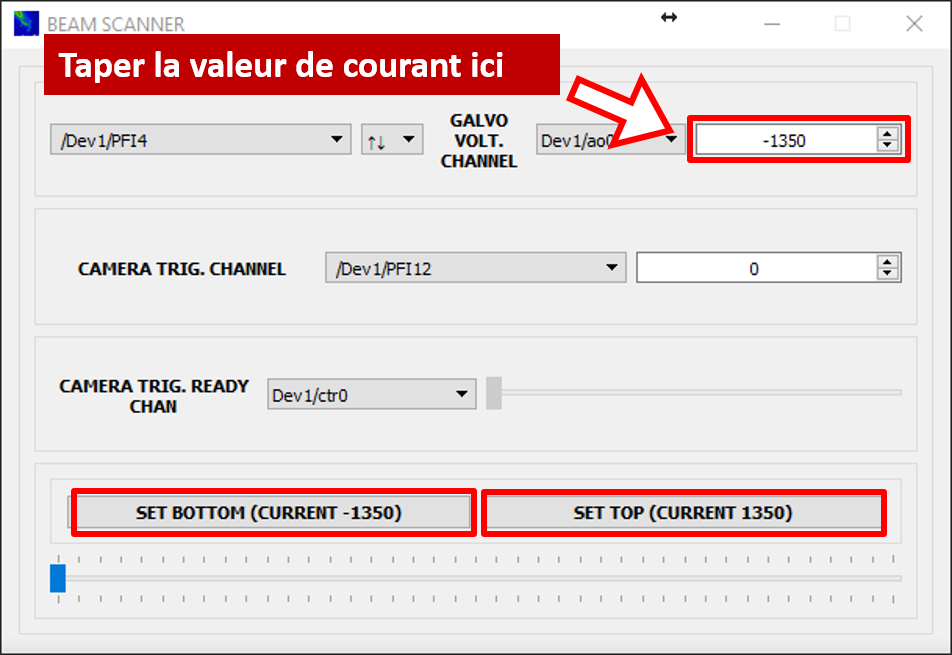
\includegraphics[width=10cm]{current.png}
        \caption{Fenêtre pop-up \textit{Scan. and. Trig.}}
        \label{fig:courant}
        \end{figure}
    \item Taper '1100' et cliquer sur \textit{Set Top (current 1000)}. Noter que la bande noire est plus étroite.
    \item Répéter l'étape précédente jusqu'à ce que la bande noire disparaisse. On veut que la bande lumineuse se rende jusqu'au rebord de l'écran sans toutefois trop dépasser. Trop dépasser entraîne une perte de puissance (i.e. fluorescence non captée par la caméra) et une acquisition de données plus longue. La valeur du courant est normalement entre 1200 et 1400.
    \item Sélectionner la limite inférieure de courant de la même façon que la limite supérieure vient d'être sélectionnée. Taper la valeur dans la même boîte. Attention: la valeur est négative; elle est normalement entre -1400 et -1200. Utiliser le bouton \textit{Set Bottom (current \#\#\#\#)}.
    \item Cliquer sur X pour fermer la fenêtre.
\end{enumerate}